\section{Tecnología}
En esta sección se va a analizar las herramientas y tecnologías empleadas en
el proyecto. La sección ha sido dividida entre software y hardware debido a que
ambas presentan gran importancia en el proyecto.

\subsection{Software}
Se han empleado una gran variedad de tecnologías, y por lo tanto, se han usado
diferentes \gls{ide} para realizar el desarrollo. Se ha empleado el lenguaje
Java para desarrollar las aplicaciones vehiculares y ciclistas, aunque
diferentes \gls{api}s, el lenguaje C para programar el microcontrolador y
para desarrollar las simulaciones de los algoritmos de previsión de accidentes
se ha empleado el JavaScript, HTML y CSS.

Para el desarrollo de las aplicaciones vehiculares se ha empleado Java con la
\gls{api} que provee NEC para desarrollar con los microcomputadores
Linkbird-MX. Para realizar las funcionalidades de \emph{logging} se ha usado
la librería \emph{log4j} de Apache. Se ha empleado la notación \gls{json} para
el envío de mensajes, para facilitar el manejo de este tipo de cadenas se ha
usado la librería \emph{JSON-java} realizada por el usuario de GitHub
Stleary. Para automatizar todas las tareas de compilación, distribución y
despliegue se ha usado la herramienta Ant de Apache ya que es multiplataforma,
ligera y soporta emplear librerias locales de forma sencilla.

La aplicación en la nube ha sido también desarrollada en Java, aunque para
facilitar el manejo de \emph{servlets} se ha empleado la libreria \emph{Jetty}.
Esta librería esta publicada por la Fundación Eclipse como software libre
bajo la licencia Apache 2.0. La ventaja de Jetty sobre otras librerías es que
es empotrable para poder ofrecer servicios Web sin requerir más dependencias,
lo cual facilita su despliegue.

Las aplicaciónes de ciclista y el \gls{hmi} del vehículo ha sido desarrollado
en el lenguaje Java, pero utilizando la \gls{api} de Android. Este \gls{sdk}
permite realizar aplicaciones móviles para el sistema operativo Android; el
cual es el sistema más extendido en el mercado. Para la comunicación de los
ciclistas con la nube mediante comunicación \emph{push} se ha empleado la
\gls{api} \gls{gcm}, lo cual permite enviar mensajes a los ciclistas sin
peligro de que pierdan una notificación si en algún momento pierden la
cobertura.

Se ha empleado el editor IntelliJ IDEA para realizar el desarrollo en Java por
las avanzadas funciones que posee de navegación de código. Este editor ha sido
realizado por JetBrains, quien ha publicado este programa en dos distribuciones:
una de pago y otra OpenSource. Se ha empleado la versión de la comunidad,
aunque por formar parte del colectivo de estudiantes ofrecen licencias de la
versión de pago de forma gratuita mientras se realicen los estudios.

Para procesar y analizar los datos que se obtuvieron durante las pruebas se ha
empleado Python 2.7, con las librerías \emph{matplotlib}, \emph{numpy} y
\emph{geopy}, para realizar una aplicación que realice el procesamiento de
los datos obtenidos y generar a partir de ellos unas gráficas. Para realizar
el \gls{ui} se ha empleado \emph{Qt4} ya que es multiplataforma y permite
el desarrollo con Python. Se ha dibujado las ventanas con QtDesigner y se ha
empleado la librería \emph{PyQt4} para gestionar las ventanas desde Python. Para
el desarrollo en Python se ha empleado el editor Sublime Text 2 por su
simplicidad, las utilidades para gestionar el código y ya que recalca el léxico
del lenguaje.

El desarrollo en el microcontrolador ha sido realizado en lenguaje C a través
del \gls{ide} y las herramientas provistas por Texas Instruments. Concretamente
se ha usado como \gls{ide} el software IAR 9.1, para flashear las aplicaciones
realizadas en la \gls{rom} se ha empleado SmartRF Flasher Programmer y para
testear las aplicaciones se ha usado las aplicacines RF Studio y Packet Sniffer.

Para validar los algoritmos desarrollados para la previsión de accidentes, se
ha realizado una simulación empleando HTML, CSS y JavaScript. Para facilitar
la escritura del código JavaScript se ha empleado el \emph{framework} JQuery,
el cual facilita tanto la gestión de las interacciones del usuario como la
modificación de elementos en la \gls{ui}. Se ha empleado el editor Visual
Studio Code para trabajar en esta parte, ya que es un editor sencillo, ligero
y que posee resaltación del léxico de los lenguajes empleados. Este editor ha
sido realizado por Microsoft y está disponible públicamente en Windows,
GNU/Linux y Mac OS X.

Las simulaciones han sido realizadas con el simulador Sumo, el cual ha sido
elegido ya que es Open Source. Esta aplicación incorpora simulaciones de
tráfico basados en algoritmos realistas, aplicaciones que permiten mejorar la
generación de redes, así como importar y exportar lostrabajos a otros
simuladores. También se ha empleado el software ns-3, el cual se trata de un
programa que provee de simulaciones con un conjunto de modelos wireless, con
distintos modelos de propagación así como diferentes implementaciones de
protocolos de acceso al medio de la familia 802.11. Este simulador
puede emplearse para ampliar las funciones de otros simuladores de movilidad.

Como repositorio del código, Mobility posee un servidor propio donde existe
instalado GitLab. Este gestor de respositorios está distribuido como software
libre y permite una sencilla gestión del código a través del software Git.

Para realizar los modelos en \gls{uml} se ha la aplicación StarUML, la cual
se distribuye de forma gratuita como \emph{shareware} con el único inconveniente
de que aparece una ventana ofreciendo la versión completa cada cierto tiempo.
Para desarrollar otros diagramas y figuras se ha empleado LibreOffice Draw y
Gimp. Para la gestión de tiempos del proyecto se ha empleado Microsoft Project
que ofrece a los estudiantes la Universidad de Deusto; ya que es la plataforma
recomendada por la universidad para este fin.

En la estación de trabajo se ha empleado el sistema operativo \emph{Debian
Testing} para trabajar ya que se deseaba emplear tecnologías libres durante
todo el desarrollo. Además, en este sistema operativo la gestión de paquetes
se realiza de forma más sencilla, por lo que las dependencias de librerías de
desarrollo que se han requerido se han resuelto de forma rápida; ya que se
integran rápidamente en el sistema. Tan solo se ha requerido emplear el sistema
operativo Windows 8, el cual provee DeustoTech, para realizar el desarrollo
del microcontrolador ya que Texas Instruments tan solo distribuye sus
herramientas para Windows.

\subsection{Hardware}
El hardware empleado se puede dividir en dos grupos: por un lado el hardware
empleado por el \gls{obu} y \gls{rsu}, y por el otro el casco \gls{ble} que
visten los ciclistas para saber en qué dirección se aproxima el vehículo.

El hardware que integran los vehículos y la infraestructura de las carreteras
se trata de la plataforma experimental NEC Linkbird-MX (Figura
\ref{fig:linkbird-mx}). Es un minicomputador que posee una tarjeta de red que
le permite comunicarse con otros dispositivos Linkbird-MX a través de una red
\Gls{802.11p}; a esta tarjeta de red se puede conectar dos antenas. Requiere
de un \gls{gps} \gls{usb} para recibir la posición del vehículo, aunque esta
característica es opcional, por lo que ha empleado un \gls{gps} de alta
precisión \emph{HI 204-III GPS USB} (Figura \ref{hi_204III_usb}) para equipar
el \gls{obu}.

El casco \gls{ble} posee un microcontrolador \gls{SoC} \emph{Texas Instruments
CC2540} (Figura \ref{cc2540}) para realizar aplicaciones de bajo consumo
empleando Bluetooth. Este dispositivo de bajo presupuesto permite realizar
nodos maestros o esclavos a través de \gls{ble}. Este dispositivo permite
flashear programas de hasta 128 KB, suficiente para hacer la aplicación que se
requiere en este proyecto. Aunque no se encuentre soportado oficialmente, este
dispositivo tiene varios puertos \gls{gpio}, los cuales se van a emplear para
conectar los led. Estos microcontroladores se emplean para aplicaciones donde
no se requiera gran capacidad de computo, y se necesite que exista una buena
autonomía.

\begin{figure}[h]
	\begin{center}
		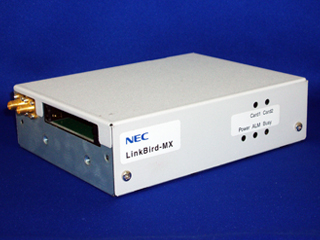
\includegraphics[scale=0.6]{linkbird-mx}
		\caption{NEC Linkbird-MX}
		\label{fig:linkbird-mx}
	\end{center}
\end{figure}

\begin{figure}[h]
	\begin{center}
		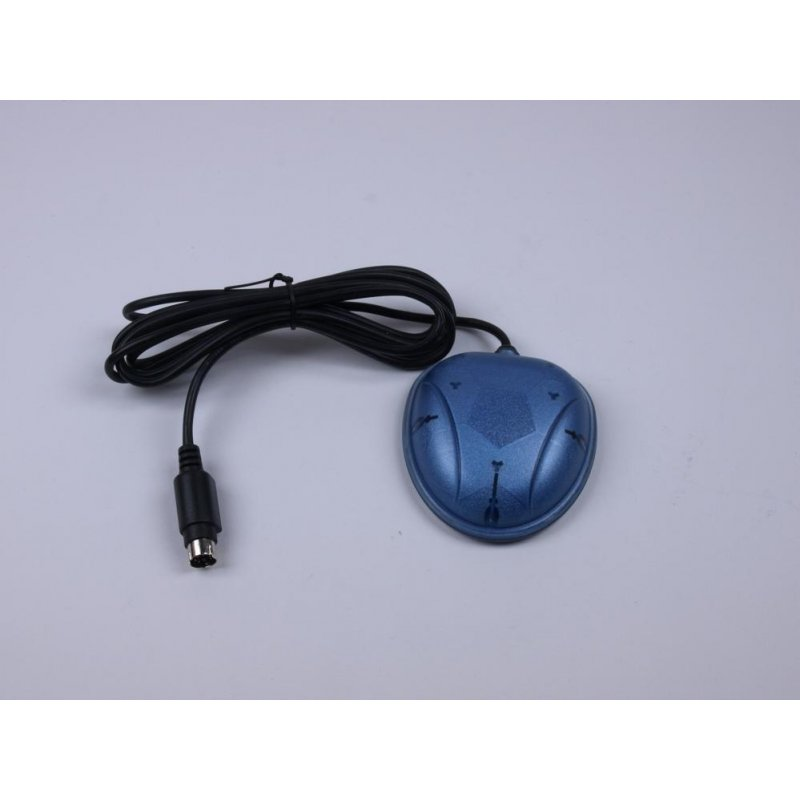
\includegraphics[scale=0.2]{hi_204III_usb}
		\caption{GPS de alta precisión HI 204-III}
		\label{fig:cc2540}
	\end{center}s
\end{figure}

\begin{figure}[h]
	\begin{center}
		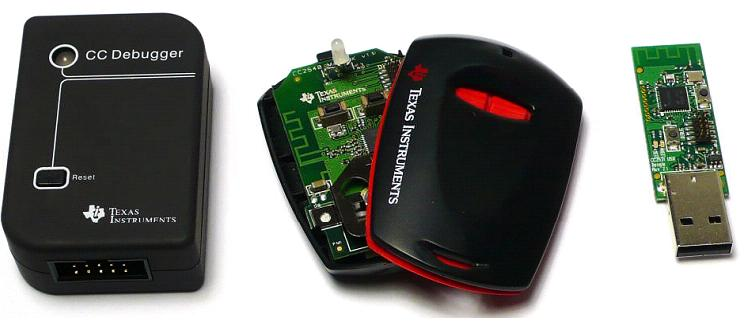
\includegraphics[scale=0.4]{cc2540dk}
		\caption{Kit de desarrollo Texas Instruments y microcontrolador CC2540}
		\label{fig:cc2540}
	\end{center}
\end{figure}
